\begin{figure}[H]
    \centering
    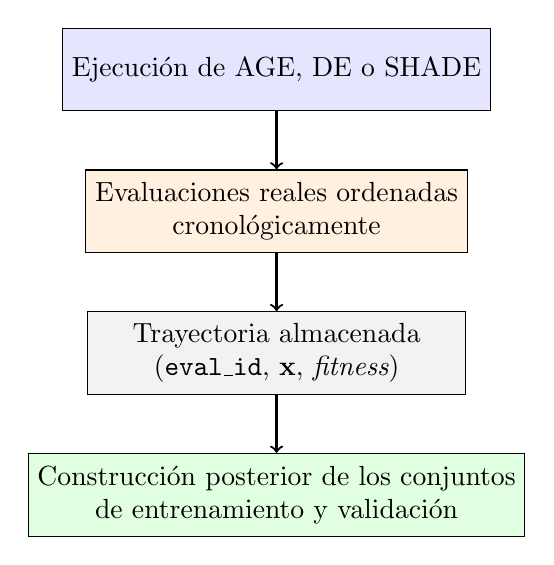
\begin{tikzpicture}[
        bloque/.style={
            draw,
            minimum width=4.8cm,
            minimum height=1.05cm,
            align=center
        },
        flecha/.style={->, thick}
    ]
        \node[bloque, fill=blue!10] (algoritmo) at (0,0)
        {Ejecución de AGE, DE o SHADE};

        \node[bloque, fill=orange!12] (evaluaciones) at (0,-1.8)
        {Evaluaciones reales ordenadas\\cronológicamente};

        \node[bloque, fill=gray!10] (trayectoria) at (0,-3.6)
        {Trayectoria almacenada\\
        \(\left(\texttt{eval\_id},\, \mathbf{x},\, \textit{fitness}\right)\)};

        \node[bloque, fill=green!12] (bloques) at (0,-5.4)
        {Construcción posterior de los conjuntos\\
        de entrenamiento y validación};

        \draw[flecha] (algoritmo.south) -- (evaluaciones.north);
        \draw[flecha] (evaluaciones.south) -- (trayectoria.north);
        \draw[flecha] (trayectoria.south) -- (bloques.north);
    \end{tikzpicture}
    \caption{Proceso de generación y registro de las trayectorias de búsqueda.}
    \label{fig:generacion_trayectorias}
\end{figure}